The physical and biogeochemical fields used to force the ecosystem model are extracted from an oceanic simulation performed with the NEMO (Nucleus for European Modelling of the Ocean; \cite{madecNEMOOceanEngine2019}) dynamical ocean model that includes the biogeochemical component PISCES (Pelagic Interaction Scheme for Carbon and Ecosystem Studies; Aumont et al., 2015). PISCES is a model of intermediate complexity designed for global ocean applications (\cite{aumontPISCESv2OceanBiogeochemical2015}), which uses 24 prognostic variables and simulates biogeochemical cycles of oxygen, carbon and the main nutrients controlling phytoplankton growth (nitrate, ammonium, phosphate, silicic acid, and iron). It simulates the lower trophic levels of marine ecosystems distinguishing four plankton functional types based on size: two phytoplankton groups (small = nanophytoplankton and large = diatoms) and two zooplankton groups (small = microzooplankton and large = mesozooplankton). The model uses the tripolar ORCA1 grid configuration (\cite{madecGlobalOceanMesh1996}), with a 1° nominal horizontal resolution with a refined 1/3° meridional resolution in the equatorial band. The vertical resolution ranges from 1 m at the surface to 100m at 1 kilometer depth.

This ocean model is forced over the 1958 to 2018 period with atmospheric inputs from JRA atmospheric reanalysis (\cite{kobayashiJRA55ReanalysisGeneral2015}), representative of observed variability over the historical period. Temperature, ocean transports, oxygen, plankton concentration (diatoms, mesozooplankton and microzooplankton, big particulate organic matter), photosynthetically active radiation (PAR) and the layer thickness from this simulation are then used to force the Apecosm ecosystem model.

Although successfully used in a variety of ENSO-related physical and biogeochemical studies in the tropical Pacific (e.g., \cite{vialardModelStudyOceanic2001, lengaigneImpactIsopycnalMixing2003, lengaigneInfluenceOceanicBiology2007, schneiderClimateinducedInterannualVariability2008, masottiLargescaleShiftsPhytoplankton2011, currieIndianOceanDipole2013}), the ability of our simulation to capture ENSO surface temperature and chlorophyll signature satellite surface Chl is briefly evaluated. 

The ONI index simulated by the model compares very well with the observed one (Fig. \ref{fig:nemo-had-sst}), with a correlation coefficient between the two time-series reaching 0.94 over their common 1958-2018 period. In particular, the model is able to accurately capture the timing and amplitude of major El Niño events, like in 1972/73, 1982/83, 1997/98 and 2015/16 and of major La Niña events, like in 1988/89 and 1999/2000. ENSO SST pattern is evaluated  by computing the covariances between the ONI and detrended monthly SST anomalies over the tropical Pacific. The covariances obtained with the Hadley Sea-Surface Temperature (HadISST1, \cite{raynerGlobalAnalysesSea2003}) anomalies and the simulated ones are shown in Fig.\ref{fig:nemo-had-sst}.

\begin{figure}
	\centering
	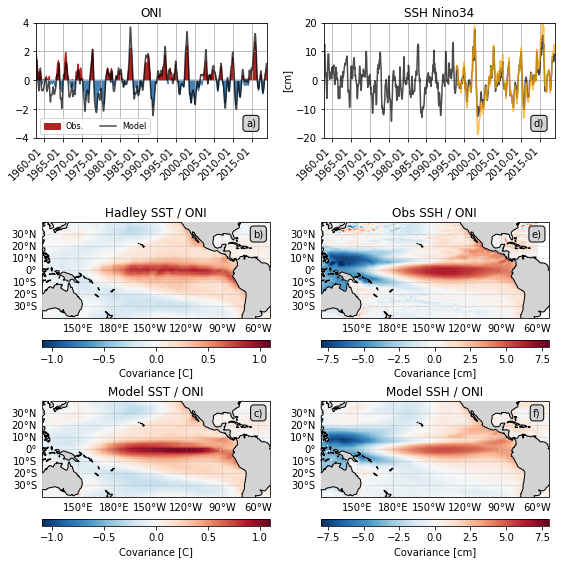
\includegraphics[scale=0.4]{figs/fig1.png}
	\caption{Simulated and observed ONI (a) and filtered TPI (b) indexes. Covariance between the Hadley SST anomalies and the ONI (c) and filtered TPI index (e). Same thing for simulated SST anomalies (d, f).}
	\label{fig:nemo-had-sst}
\end{figure}

Modelled ENSO SST  pattern closely resembles the observed one. This pattern is characterized by warm SST anomalies (1°C) centred in the central and eastern equatorial Pacific  flanked by the traditional horseshoe cooling pattern in the western Pacific extending towards the subtropical north and south Pacific. This SST seesaw in the equatorial region is further accompanied by a shoaling of the thermocline in the west and a deepening in the east (not shown).

Covariance maps between the surface chlorophyll and the monthly ONI index are shown in Fig \ref{fig:nemo-sat-chl}. The observations (upper panel), based on the  OceanColour-CCI V5 dataset \citep{sathyendranathOceanColourTimeSeries2019},  and the model (lower panel) show very similar covariance pattern: El Niño induces a decrease in chlorophyll concentration in the along the equator east of 150°E, consistent with a weaker equatorial upwelling induced by the equatorial trade winds reduction. However, the model overestimates the chlorophyll response to ENSO variability compared with observational based estimates. Note that the covariance for the simulated chlorophyll has also been computed over the entire simulated period (1958-2018), with no significant changes in the resulting pattern (not shown).

\begin{figure}
	\centering
	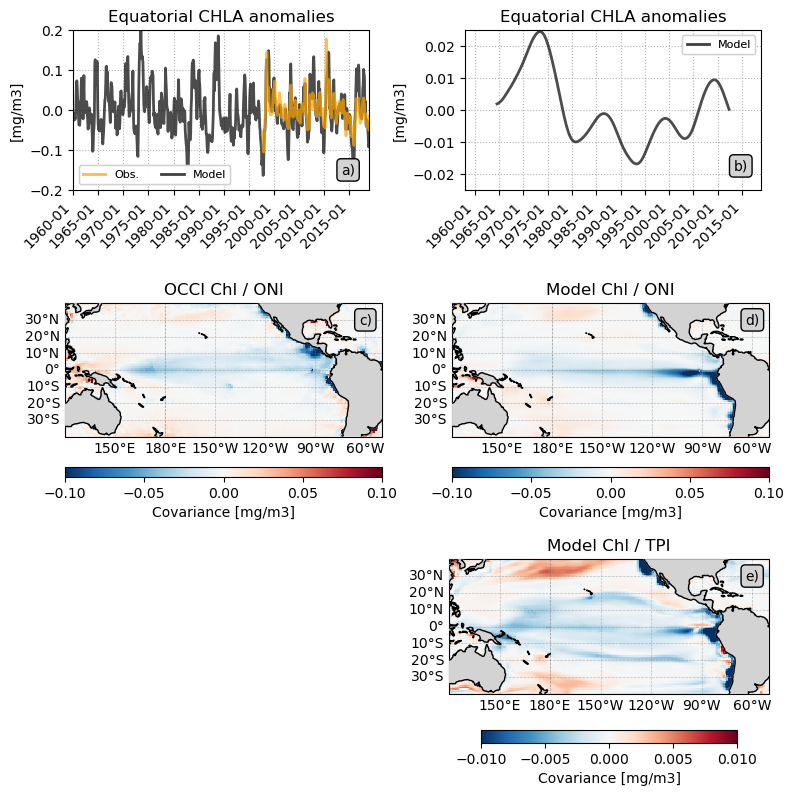
\includegraphics[scale=0.4]{figs/fig2.png}
	\caption{Simulated (black) and observed (yellow) equatorial chlorophyll anomalies (a). Filtered anomalies are shown for the model in panel (b). Covariance between the observed and simulated chlorophyll anomalies with the ONI (c, d) and filtered TPI (e) index.  }
	\label{fig:nemo-sat-chl}
\end{figure}